%
% CITI Research Report Template
%
% 07/2012: Paul Ferrand - Initial Template
% 02/2013: Frederic Le Mouel - Refactoring
% 

\documentclass[a4paper]{article}

%
  
\usepackage{pdflscape}
\usepackage{multirow}
\usepackage[utf8]{inputenc}% ou \usepackage[latin1]{inputenc}
\usepackage[T1]{fontenc}
\usepackage{lmodern}
\usepackage{graphicx}
\usepackage{listings}
\usepackage[bookmarks]{hyperref}
\usepackage{caption}
\usepackage{adjustbox}
\usepackage[section]{placeins}


\lstset{numbers=left, numberstyle=\small, numbersep=8pt, frame = single, framexleftmargin=15pt, columns=fullflexible,basicstyle=\ttfamily, breaklines=true,  tabsize=2}

\begin{document}

%
% Cover Page
%

\pagestyle{empty}
\begin{center}
\begin{figure}%
\centering
%
\includegraphics[width=0.5\columnwidth]{logo/citi-old-bw.eps}% old logo
%
\includegraphics[width=0.4\columnwidth]{logo/citi-new-bw.eps}% new logo 

\includegraphics[width=0.4\columnwidth]{logo/citi-new-title-bw.eps}% old logo - titled
\end{figure}
%{\LARGE \textsc{Communication scientifique}} \\ % in French
{\LARGE \textsc{Scientific Communication}} \\ % in English
\vspace{0.5cm}
%{Centre d'Innovation en Télécommunications et Intégration de Services} \\ % in French
{Center of Innovation in Telecommunications and Integration of Services} \\ % in English
\vspace{2cm}
{\Large \textbf{ConGolo: A Context-oriented language based on Golo}} \\
\vspace{10pt}
{\large \textit{Baptiste Maingret}} \\
\vspace{10pt}
{\large April 2014} \\
\vspace{20pt}
\begin{minipage}{0.8\columnwidth}
\sffamily
\small
INCLUDE ABSTRACT HERE
\end{minipage}
\end{center}
\vfill
\begin{minipage}[b]{0.3\columnwidth}

\includegraphics[width=\columnwidth]{logo/inria.eps}%
\end{minipage}
\hfill
\begin{minipage}{0.3\columnwidth}
\small
\centering
\textbf{
%University of Lyon \\ % in English
INSA Lyon \\ % in English
Shanghai Jiao Tong University
}
\end{minipage}
\hfill
\begin{minipage}[b]{0.25\columnwidth}

\includegraphics[width=\columnwidth]{logo/insa-noir.eps}%
\end{minipage}

\newpage

%
% Title page
%

\title{Research Report}

\author{Baptiste Maingret\\[10pt]
INSA-Lyon, F-69621, Villeurbanne, France\\
\texttt{baptiste.maingret@insa-lyon.fr}}

\date{\today}
\newcommand{\Keywords}[1]{\par\noindent 
{\small{\em Keywords\/}: Context-Oriented Programming, Golo, Java, System reasoning, Dynamic Language}}
\maketitle

\begin{abstract} 
Insert abstract here
\Keywords{Context-Oriented Programming, Golo, Java, System reasoning, Dynamic Language}
\end{abstract}

\newpage

%
% Report Body
%

\section{Introduction}

Internet of Things (IoT) takes a lot attention nowadays because of its implication in our daily lives, its market opportunitiesand also because of its unique technological requirements. Protocols have emerged to make the IoT a reality and today's trend is to standardize them to allow its further development and ease of interconnection with existing infrastructures. Thus the Web of Things is also taking interest because of the ease of development, its well-known standard and the numerous existing web-based systems. On the other side software development for IoT has not seen many improvements nor recent evolution to cope with the new specificities of IoT such as mobility, variable environment, dynamism...

In parallel context-oriented programming (COP) has drawn research interest in the past years and as a result several new COP languages have emerged. Most of these approaches allow for multiple context definitions and their activations. They also allow the developer to specify context-dependent behaviours. Because of the dynamism of the IoT, COP could be a good option for the development of IoT applications.

The decision-making systems backing up these COP languages is usually simple and may have difficulties to cop with the requirements of IoT. Whereas it is to decide what context should be activated or what actions should be done based on the current context, current systems only allow for one implementation and does not provide any sort of abstraction. Systems are often simple event-condition-action (ECA) process which do not leverage the full potential of the IoT. More advanced systems such as neural networks, genetic algorithms or Petri net could be used.

May languages have seen their COP counterparts born. Several approaches were based on Java and the JVM. Because of its high development in embedded system, the JVM seems to be a good candidate for the development of IoT applications. In addition, dynamic languages for the JVM have been created such as Groovy or Golo \cite{ponge_golo_2013}, a lightweight dynamic JVM language built around invokedynamic.

In this paper we propose a new COP language named ConGolo, extending the Golo language, and binding to a Java API that will provide an abstraction of the reasoning mechanisms, whether it is a simple event-condition-action (ECA), an automate, a neural network or yet another approach. To test our solution and put it into action, we will propose a use-case based on a WoT application.


In section \ref{section:stateoftheart} we will first see the different approaches taken by existing COP languages to explain the choices made in ConGolo. In \ref{section:contribution} we will present Congolo and the abstraction mechanism for decision-making and reasoning systems. In \ref{section:implementation} we will describe the implementation and discuss the choices made.



\section{State of the Art: Context-Oriented Programming}
\label{section:stateoftheart}
`
\paragraph{Context-Oriented Programming}
There are already many COP languages based on a variety of languages. Most of them implements the context with the use of layers which acts as a context and context-dependent behaviours definition but some others also explicitly separate the two. In order to compare these languages we can thus focus at first on the way the context are defined, then how they are activated and finally how they are used throughout the code. A summary table \ref{table:coplanguages}, inspired by \cite{appeltauer_comparison_2009}, is proposed.

In many languages, context is integrated directly in the business code by the mean of layers. It is the case in JCop \cite{appeltauer_declarative_2012}, as in listing \ref{listing:jcoplayer}, ContextJ \cite{appeltauer_dedicated_2008} \cite{appeltauer_improving_2009}, ContextErlang \cite{ghezzi_context_2010}, ContextLua \cite{wasty_contextlua:_2010} or EventCJ \cite{kamina_eventcj:_2011}. In ECaesarJ \cite{nunez_declarative_2009}, NextEJ \cite{kamina_towards_2009} or Javanese \cite{kamina_unified_2013} the contexts are declared separately as in listings \ref{listing:ecaesarjcontext}, \ref{listing:javanesecontext} and \ref{listing:nextejcontext}. In EventJava \cite{jayaram_context-oriented_2009}, context is considered to be an event with specific data, listing \ref{listing:eventjavacontext} and is defined alongside the event consumer. Thus when the event arrives, the context is embedded into it.

\begin{lstlisting}[float, language=Java, caption=JCop layer example, label={listing:jcoplayer}]
public class Hero {
  public Point getPosition() {...} //plain meth.
  public void move(Direction dir) {...} //base meth. for layered method Hero.move
  private Position getPos() {...} //base meth. for layered method Hero.getPos
  
  layer ConfusedHeroLayer { //layer extension declaration
    private Position getPos() {...} //partial meth. for layered method Hero.getPos
  }

  public layer ConfusedHeroLayer { //(top-level) layer declaration
    public void Hero.move(Direction dir) { //partial meth. for layerd meth. Hero.move
      proceed(dir); //a proceed expression
    }
    private Direction getNewDir(Direction original) {...} //layer local method
  }
}
\end{lstlisting}

\begin{lstlisting}[float, language=Java, caption=ECaesarJ context declaration, label={listing:ecaesarjcontext}]
cclass ScheduledNightTime extends Context {
  TimeService sunset, sunrise;
  event in() = sunset.time();
  event out() = execution(* *.openBinds(..));
  // or
  //  event out() = sensor.intensityChanged(int i) && if (isActive() && i > threshold);
}
\end{lstlisting}

\begin{lstlisting}[float, language=Java, caption=Javanese context declaration, label={listing:javanesecontext}]
// Contexts declaration
context GPSon
  active(int s) :after call(void Nav.onStatusChanged(*)) && args(s)
      && if(GPS.AVAILABLE==s)
  until(int s) :after call(void Nav.onStatusChanged(*)) && args(s)
      && if(GPS.AVAILABLE!=s);
      
context RouteSearching
  // context active during the execution of the specified method
  cflow(call(void Nav.calcRoute()));
\end{lstlisting}

\begin{lstlisting}[float, language=Java, caption=NextEJ context declaration, label={listing:nextejcontext}]
context Building {
  role Guest {
    void escape() { .. }
  }
  role Security {
    void notify() {
      Guest.escape();
    }
  }
}
\end{lstlisting}

\begin{lstlisting}[float, language=Java, caption=EventJava context declaration, label={listing:eventjavacontext}]
public class Context implements Comparable<Context>, Serializable {
  public long time;
  ... /* more fields */
  public Context() { time = System.currentTimeMillis(); }
  public Context(long time) { this.time = time; }
  public int compare(Context other) {
    if(timestamp == other.timestamp) return 0;
    ...
  }
  ...
}
\end{lstlisting}

The activation of the context, or layers depending on the language, often use the keyword \lstinline|with| \cite{haupt_contextj:_2011} \cite{appeltauer_declarative_2013} \cite{kamina_towards_2009} \cite{wasty_contextlua:_2010} as shown in the listing \ref{listing:jcopwith}. Instead \cite{ghezzi_context_2010}, \cite{nunez_declarative_2009} or \cite{kamina_eventcj:_2011} use a different approach where contexts are activated independently of the running program by the mean of events. In \cite{nunez_declarative_2009}, the activation is done by the use of specific events declared in the context object which can be triggered by others events, by method invocation or by composite expression as in listing \ref{listing:ecaesarjcontext}. In \cite{kamina_eventcj:_2011}, they declare transition rules based on events that will activate or deactivate contexts, as in listing \ref{listing:eventcjevent}. In \cite{kamina_unified_2013}, where the distinction is made between context and layers, the context state is changed by specific actions and thus can be activate in the program, whereas layers are activated according to the state of one or multiple contexts and thus are activated implicitly, as in listing \ref{listing:javanesecontext}. Finally in \cite{jayaram_context-oriented_2009} where the context is defined by specific values of information when the event is triggered, the activation of the context is global but its particular definition, i.e. the values of the information that it holds, are defined by events.

 
\begin{lstlisting}[float, language=Java, caption=JCop layer activation, label={listing:jcopwith}]
public void moveHeroLeft() {
	with (new ConfusedHeroLayer(), new RainLayer()) {
    getHero().move(Direction.LEFT); }
}
\end{lstlisting}

\begin{lstlisting}[float, language=Java, caption=EventCJ layer activation, label={listing:eventcjevent}]
direction SwitchPositioningDevice {
  declare event GPSEvent(Navigation n, int s)
    :after call(void Navigation.onStatusChanged(s))
      &&target(n)&&args(s)
      &&if(s==LocationProvider.AVAILABLE)
    :sendTo(n);
  declare event WifiEvent(Navigation n, int s)
    :after call(void Navigation.onStatusChanged(s))
      &&target(n)&&args(s)
      &&if(s==LocationProvider.OUT_OF_SERVICE)
    :sendTo(n);
  declare event Boarding()
    :after call(void *.cabinModeEntered());
  declare event Arriving()
    :after call(void *.cabinModeExit());
  
  transition GPSEvent:
    WifiNavi switchTo GPSNavi | not OnBoard activate GPSNavi;
  transition WifiEvent:
    GPSNavi switchTo WifiNavi | not OnBoard activate WifiNavi;
  transition Boarding:
    * switchTo OnBoard;
  transition Arriving:
    OnBoard switchTo .;
}
\end{lstlisting}

\begin{lstlisting}[float, language=Java, caption=Javanese context declaration, label={listing:javaneselayer}]
// Layers declaration
activate Outdoors when GPSon && StrongGPS;
activate Indoors when !GPSon || !StrongGPS;
\end{lstlisting}

Finally, we need to consider how the rest of the program takes into account the different contexts to adapt and modify the program. Two strategies are often found when the language use a layer paradigm: layer-in-class and class-in-layer implementation, but only the first one is usually implemented. In the first one, the layers and corresponding behaviours are implemented inside the class such as in \cite{appeltauer_improving_2009} \cite{appeltauer_declarative_2013} \cite{wasty_contextlua:_2010} (listing \ref{listing:jcoplayer}) or as in \cite{kamina_eventcj:_2011} \cite{kamina_unified_2013} (listing \ref{listing:eventcjlayeruse}). \cite{kamina_towards_2009} follows the same approach but differs by the fact that thev use roles defined in the context classes to implement the different behaviours. \cite{ghezzi_context_2010} states that both methods have their advantages and thus offers the possibility of using the both of them. ECaesarJ offers two distinct ways of using the current context. First, it is possible to bind specific events to the events triggered by the context changes as in listing \ref{listing:ecaesarjcontextuse} or to directly query the context state with the help of the method \lstinline|isActive()| of the context. In \cite{jayaram_context-oriented_2009}, as the context is represented by variables bound to an events, the context-dependent behaviours are implemented using this data such as in listing \ref{listing:eventjavacontextuse}.

\begin{lstlisting}[float, language=Java, caption=ECaesarJ context use, label={listing:ecaesarjcontextuse}]
cclass LightAutomation {
  ILight light;
  Context context;

  event mustTurnOn() = context.in();
  event mustTurnOff() = context.out();

  mustTurnOn() => { light.switchOn(); }
  mustTurnOff() => { light.switchOff(); }
}
\end{lstlisting}

\begin{lstlisting}[float, language=Java, caption=EventCJ context-dependent behaviour, label={listing:eventcjlayeruse}]
class Navigation extends MapActivity implements Runnable, LocationListener {
  MapView mapView;
  MyLocationOverlay overlay;
    
  void onStatusChanged(...) {...}
  void run() {}
  void onCreate(Bundle status) {
    overlay.runOnFirstFix(this);
  }
  
  layer GPSNavi {
    activate { overlay.onProviderEnabled("gps"); }
    deactivate { overlay.onProviderDisabled("gps"); }
    after void run() {
      Location loc = overlay.getMyLocation();
      mapView.getController().animateTo(loc);
  }
}
\end{lstlisting}

\begin{lstlisting}[float, language=Java, caption=EventJava context-dependent behaviour, label={listing:eventjavacontextuse}]
public class Context implements Comparable<Context> , Serializable {
	public long time;
	public float latitude; //in decimal degree format
	public float longitude; //in decimal degree format
	... //more fields and methods
}

class AnimalMonitor1 {
	float currLatitude;
	float currLongitude;
	2DPoint loc = new 2DPoint(currLatitude, currLongitude);
	event animalLocation[10](long animalID, String family) when
		( for i in 0..8 animalLocation[i].animalID == animalLocation[i+1].animalID &&
		for i in 0..9 euclideanDistance(loc, new 2DPoint(animalLocation[i].latitude, animalLocation[i].longitude)) > 0.5 &&
		animalLocation[9].time - animalLocation[0].time <= 60*60*1000) {
			triggerAlert("Animal " + animalID + " out of safety zone ");
		}
}
\end{lstlisting}

There exist different type of implementation for COP languages. The easiest one might be to develop an API such as \cite{appeltauer_dedicated_2008}. One can also extends existing languages with new keywords such as in \cite{clarke_semantics_2009}, ContextJ \cite{haupt_contextj:_2011}, JCOP \cite{appeltauer_declarative_2013}, NextEJ \cite{kamina_towards_2009} or \cite{ghezzi_context_2010}. Finally some papers propose a new COP language as  EventCJ \cite{kamina_eventcj:_2011} or \cite{kamina_unified_2013}.

\begin{landscape}
  \begin{table}
  \begin{adjustbox}{center}
  \begin{tabular}{l p{3cm} c c c c c c c c c c}
  \hline
  \multicolumn{2}{l}{Languages} & ContextJ & JCop & EventCJ & NextEJ & ContextLua & ContextErlang & EventJava & Javanese & ECaesarJ \\

  \hline
  \multirow{2}{*}{Context declaration}
    & Layer &   X & X & - & - & X & X & - & - & - \\
    & Class &   - & - & X & X & - & - & X & X & X \\

  \hline  
  \multirow{2}{*}{Layer declaration}
    & Layer-in-class &   X & X & X & X & X & X & X & X & X \\
    & Class-in-layer &   - & - & - & - & - & X & - & - & - \\

  \hline
  \multirow{2}{*}{Layer implementation}
    & Class &       - & - & - & - & - & - & - & X & X \\
    & Layer type &  X & X & X & X & X & - & - & X & - \\    

  \hline  
  \multirow{3}{*}{Scope}
    & Instance &        - & - & X & - & X & - & X & X & X \\
    & Thread &          X & X & - & - & - & - & X & X & - \\
    & Dynamic extent &    &   &   &   &   &   &   &   &   \\
    & Global &          - & - & - & - & - & X & X & X & - \\

  \hline
  \multicolumn{2}{l}{Events/messages supported}
    & - & - & X & - & - & - & X & X & X \\

  \hline
  \multirow{2}{*}{Active context tracking}
    & Push to layer stack &             X & X & X & - & - & X & X & X & - \\
    & Directly change method lookup &   - & - & - & - & - & - & X & - & - \\

  \hline    
  \multirow{3}{*}{Implementation}
    & Language extension &   X & X & - & - & X & X & X & X & - \\
    & New language &         - & - & X & - & - & - & - & X & - \\

  \end{tabular}
  \end{adjustbox}
  \caption{COP languages comparison}
  \label{table:coplanguages}

  \end{table}
\end{landscape}


\paragraph{Decision-making systems}
Decision making is the process of outputting a final choice based on inputs, that could result in an action. There exist several approaches that we can at first separate into two groups based: fixed-design and machine learning.

Basic systems such as event-condition-action (ECA), state transition systems or Petri net allow basic decision making. They do not require any training and only a basic initialization. In most of the COP languages cited above, ECA is used for the layers activation.

More advanced systems of machine learning can be used for decision making. These include artificial Bayesian networks, cluster analysis techniques, particle swarm, simulated annealing, support vector machine, decision-tree learning, association rule learning, similarity and metric learning, sparse dictionary learning, artificial neural networks (ANN), genetic algorithms... They usually are classified in three categories, each of them allowed to belong to more than one, based on the type of learning that can be used to initialize the system: supervised, unsupervised and reinforcement \ref{table:machinelearning}.

\begin{table}[bt]
\begin{tabular}{l c c c }
\hline
\multirow{2}{*}{Languages} & \multicolumn{3}{c}{Learning method} \\

 & Supervised	 & Unsupervised	& Reinforcement \\

\hline
Bayesian Networks	             & X & - & - \\

\hline
Clustering	                     & - & X & - \\

\hline
Genetic Algorithms             & - & - & X \\

\hline
Artificial Neural Networks     & X & X & X \\

\hline
Particle Swarm Optimization    & X & - &	- \\

\hline
Simulated Annealing            & X & - &	- \\

\hline
Support Vector Machines        & X & - & - \\

\hline
Decision Tree Learning         & X & - &	- \\

\hline
Association Rule Learning      & - &	X &	- \\

\hline
Similarity and Metric Learning & X &	- &	- \\

\hline
Sparse Dictionary Learning     & X & X &	- \\
\end{tabular}

  \caption{Machine learning methods}
  \label{table:machinelearning}
\end{table} 

\end{table} 

From an implementation point of view, there are languages which are often used for artificial intelligence development and thus tend to be used to design decision making systems. Such languages include Lisp and its derivatives, and Prolog. However none of them include context-oriented functionnalities and there does not seem any extension for COP to exist even if aspect oriented have been researched using Prolog \cite{lohmann_aspect-oriented_2008}. In addition to these dedicated languages, there exist AI frameworks such as the Encog Machine Learning Framework (EMLF) which implements a wide variety of AI process but they still do not allow for an abstraction regarding the type of algorithm to be used.

  \section{Contribution}
\label{section:contribution}

In this paper we propose a new COP language, namely ConGolo, based on Golo language. We offer COP functionnalities based on the study of previous papers and existing solutions. We also introduce a new way of abstracting the decision making process with the help of a Java API.

\subsection{Context management}
\label{subsection:contextmanagement}

As seen in section \ref{section:stateoftheart}, most papers handle context as a simple state systems where contexts are two-state variables that can either be activated or deactivated, even if some others have different views such as the context being a data. In our case, we decided to allow a more flexible way of handling the context by introducing two levels of context values: meta-values and concrete values. The meta values are used into the business code to declare the different layers (to be understood as defined by other papers). On the other hand, concrete values are used inside the decision-maker that will output the meta values and thus decide which layers to activate, as in Figure \ref{figure:concretemetavalues}. Hence the context is not directly activated but concrete values are used to determine, with the help of a decision-maker, which context is to be activated. The current state of the context is thus represented by the current concrete values whose scope can be per-instance or global.

\begin{lstlisting}[float, language=Java, caption=ConGolo context example, label={listing:congolocontext}]
context ConfusedHero =  [
  [TRUE, FALSE],
  [alertness, sleep, stamina]

context Weather = [
  [RAINY, SUNNY],
  [luminosity, rain, temperature, humidity]
]
\end{lstlisting}

\begin{center}
\begin{figure}
\centering
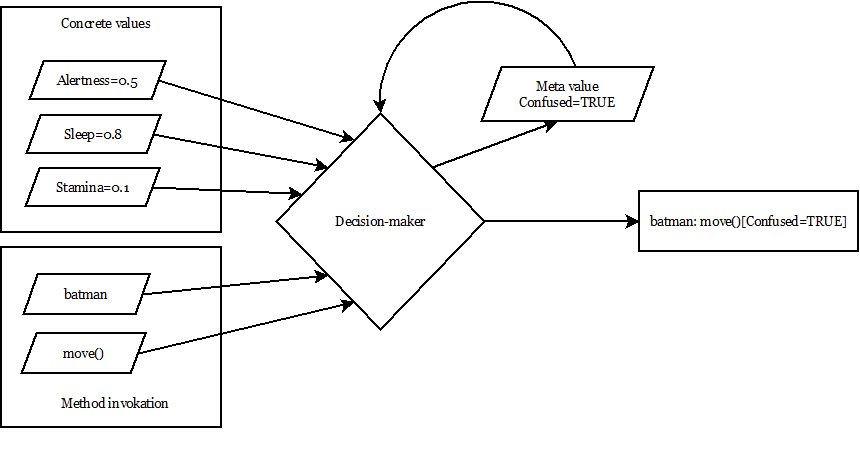
\includegraphics[width=0.9\columnwidth]{images/concrete-meta-values.png}
\caption{Concrete and meta values in context representation}
\label{figure:concretemetavalues}
\end{figure}
\end{center}

\subsection{Layers}
\label{subsection:layers}
Layers are usually defined as alternative methods to base methods (context independent) that will eventually be triggered depending on the context. The declaration is done with the help of a keyword such as \lstinline|layer|, allowing to define multiple methods belonging to one layer. In our case, we propose an alternate method definition to indicate the layer by using the square bracket symbols and appending them at the method's parameter list: \lstinline!function myFunc = |arg1|[contextA=METAVALUE1]!. This choice was made because of the compatibility of this definition with the different function definition allowed by Golo and because we think it looks like it really belongs to the language rather than having been added in an ad-hoc manner.

When multiple layers are activated at the same time, the usual proposed way is to simply take them in a LIFO manner as if they were stacked. However in our case the method to be called is chosen by the decision-maker. Thus in the case were multiple contexts, i.e. multiple meta-values, are activated at the same time, again the system will make the decision to chose which methods are to be called.

\begin{lstlisting}[float, language=Java, caption=ConGolo layers example, label={listing:congololayers}]
function Hero = || {
  return DynamicObject():
    define("getPosition", |this| -> ...): # plain method
    define("move", |this, dir| -> ...):   # base method
    define("getPos"; |this| -> ...):    # base method
    define("getPos", |this, direction|[ConfusedHero=true]+ -> ...): #layer declaration, invoked before base method
    define("move", |this, dir|+[ConfusedHero=true] -> ...):   # layer method, invoked after base method
}
\end{lstlisting}

\subsection{Decision maker}
\label{subsection:decisionmaker}

One singular aspect of our proposition regarding previous ones is the way the layers are activated. It iusually done in an ECA manner: when a specific context is activated and that a layered method is invoke, the corresponding layer is used. The decision is made at the programming stage. It is of course possible to dynamically change the context at runtime but its binding to the layers is static. What we propose is to delegate this decision to an external system, the decision-maker, which could be static just as in others papers but could also be based on more advanced algorithms and techniques such as neural networks or bayesian networks. In this case, the system could actively learn during the runtime of the application. In order to fully integrate this into the language we propose new keywords to be used in ConGolo in order to manipulate and use this system:

\begin{description}
  \item[init] Init the decision maker
  \item[train] Train the decision maker (does nothing if not available)
  \item[default] Set the decision-maker as the default ont
  \item[do] Pass the method invokation to the specified decision-maker, or the default one if omitted
  \item[dowith] Pass the method invokation to the specified decision-maker
\end{description}

\begin{lstlisting}[float, language=Java, caption=ConGolo example, label={listing:congolohero}]
let batman = Hero()   # Context-dependent object
batman: move()        # Call to a layer method directly

let decisionMaker = MyDecisionMaker() # New decision maker
init decisionMaker    # Init the decision maker using embedded keyword
train decisionMaker   # Init the decision maker using embedded keyword
default decisionMaker # Set this decision maker as the default one

do batman: move()	# Use the default decision-maker to invoke the correct method move of Hero

do {	# Support for consise multiple invokations
	batman: move()
	batman: move()
}

do {
	batman: move()
} with (decisionMaker) # Explicitely specify the decision-maker to use

dowith(decisionMaker) batman: move()	# Explicitely specify the decision-maker to use in a consise form
\end{lstlisting}

Usually these algorithms take multiple inputs and provide an output. In order to have a compatibility between these systems so that we can change it without having to redefine the entire applications we proposed that inputs would be events. This events can either contains data, such as data from the concrete values, object and method for method invokation, or context information (meta values). Thus all of these will be the inputs of the different decision-making systems, whatever the underlying implementation. As for the ouput, it can either be a method invokation, corresponding to the decision made by the system, or an event that could be further used as an input for the system.

\section{Implementation}
\label{section:implementation}
public class MyDecisionMaker implements DecisionMakerAPI {
  public void init() { ... }
  public void train() { ... }
  public void decide() { ... }
}

Detail implementation
context storage -> Java API

\section{Results}
\label{section:results}

Perfomance evaluation
10 methods layered and plain implementation as in \cite{appeltauer_comparison_2009} where multiple languages were tested to create a benchmark, similar to \cite{kamina_eventcj:_2011}.

Evaluation of COP languages and approaches are usually based on the runtime overhead or the ease of programming. The first implementation of ContextJ \cite{haupt_contextj:_2011} shown a significant overhead when using layers. In \cite{appeltauer_layered_2010} the authors explores the use of the new INVOKEDYNAMIC (ID) instruction introduced in Java 7 which allows for dynamic method dispatch to implement the layer method dispatch in JCOP \cite{appeltauer_declarative_2013}. The performances shown are encouraging especially since at the time of writing the implementation of in the JVM was not yet over. Thus the Golo language, based on ID form day one, could be a good applicant for COP languages. Regarding the other approach of evaluation which would be the ease of programming, including code duplication and code overhead, \cite{appeltauer_declarative_2013} compare JCOP to the previous ContextJ and notice a significant reduction of code due to layer inheritance mechanism and context classes to better compose layers.

\section{Conclusion \& Perspectives}
\label{section:conclusion}


%
% Bibliography
%

\bibliographystyle{plain}
\bibliography{bmaingret_PFE_2014_Report}


\end{document}

